\section{Chapter 1 - Circuit Variables}

\subsection{Electrical Engineering - An Overview}

This section is primarily a vocabulary only based section so there are no example problems.

\subsection{Units}

Assume a telephone travels through a cable at two-thirds the speed of light.
How long does it take the signal to get from New York City to Miami if the distance is
approximately 1100 miles? \\We know

\begin{itemize}
	\item The speed of light is 3\e{8} m/s
	\item There are 1.6 km in a mile
	\item There are 1,000 meters in a kilometer
\end{itemize}

\begin{align*}
	&= \left(\frac{second}{\frac{2}{3}\times 3\e{8} meters}\right)\times \left(\frac{1.6 km}{mile}\right) \times \left(\frac{1000 m}{km}\right) \times 1100 miles
	\\ &= \left(\frac{second}{\frac{2}{3}\times 3\e{8} \cancel{meters}}\right) \times \left(\frac{1.6 \cancel{km}}{\cancel{mile}}\right) \times \left(\frac{1000 \cancel{meters}}{\cancel{km}}\right) \times 1100 \cancel{miles}
	\\ &= \frac{1.6 \times 1000 \times 1100 \times seconds}{\frac{2}{3} \times 3\e{8}}
	\\ &= \frac{1760000}{2e{8}}
	\\ &= 0.0088 seconds
	\\ &= 8.8 ms
\end{align*}

\newpage
\subsection{Voltage, Current, Power, and Energy}
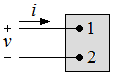
\includegraphics{img/c1/idealbasiccircuit}

The current at the terminals of the element in the above diagram is:

\begin{itemize}
	\item \( i = 0, t < 0 \)
	\item \( i = 20e^{-5000t}, t\geq0 \)
\end{itemize}

Calculate the total charge (in microcoulombs) entering the element at its upper terminal.
\\ We know the equation for current is:

\( i = \frac{dq}{dt} \)
Therefore the equation for total charge is:

\( q(t) =  \int_{0}^{t}i(x)dx \)

To find the total charge we need to find the current from 0, to \( \infty \). Substituing our equation
for i and we get:

\(q_{total} = \int_{0}^{\infty}20e^{(-5000t)}dx \)

The solving we get:

\begin{align*}
	q_{total} &= \frac{20}{-5000}e^{-5000x} \Big|_{0}^{\infty}
	\\ q_{total} &= \frac{20}{-5000}\left(e^{-\infty} - e^{0}\right)
	\\ q_{total} &= \frac{20}{-5000}\left(0 - 1\right)
	\\ q_{total} &= \frac{20}{-5000}
	\\ q_{total} &= 0.004 C
	\\ q_{total} &= 4000 \mu C
\end{align*}
 
\newpage
\subsection{Voltage, Current, Power, and Energy}
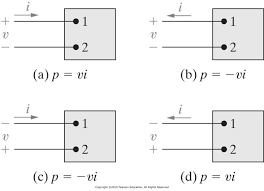
\includegraphics{img/c1/power}

Assume that a 20 V voltage drop occurs across an element from terminal 2 to terminal 1 and
that a current of 4 A enters terminal 2.

\begin{enumerate}
	\item Specify the values of v and i for the polarity references shown in the figure above.
	\item State whether the circuit inside the box is absorbing or delivering power.
	\item How much power is the circuit absorbing? 
\end{enumerate}

1) We are told the positive terminal is connected to terminal 2, and the negative terminal is
connected to terminal 1. We are also told that a current of 4 A enters terminal 2. 
a) The positive terminal is connected to terminal 2 which means the voltage is negatively referenced.
The current is referenced entering terminal 1, but our current is entering terminal 2. Therefore the current is negatively referenced. \(v = -20V \) , \(i = -4A\)
\\b) The positive terminal is connected to terminal 2  which means the voltage is negatively
referenced. The current is referenced leaving terminal 1, and our current is referenced entering
terminal 2, which means the current is positively referenced. \(v = -20V \), \(i = 4A\)
\\c) The positive terminal is connected to terminal 2, which is also the positive reference. 
Therefore voltage will be positive. The current is referenced as entering terminal 1, but our current is entering terminal 2. Therefore the current is negatively referenced. \(v = 20V\), \(i = -4A\)
\\d) The positive terminal is connected to the positive reference point. The current is flowing
in the appropriate direction. Therefore both the voltage and the current are positively referenced.
\(v = 20V\), \(i=4A\)
\\2) We will use the reference shown in Figure (a). Using the passive sign convention we can see that
the voltage and the current will be negative. Therefore:

\begin{align*}
	p &= v \times i
	\\ p &= (-20) \times (-4)
	\\ p &= 80W
\end{align*}
Because the power is greater than 0, the box is absorbing power. 
\\3) We can see from the calculation above that the box is absorbing 80 W

\newpage
\subsection{Voltage, Current, Power, and Energy}

Find the current drawn from a 115-V line by a dc electric motor that delivers 1 hp. Assume
100\% efficency. 

\begin{align*}
	P &= VI
	\\ I &= \frac{P}{V}
	\\ 1 hp &= 745.7 W
	\\ I &= \left( \frac{1 hp}{115 V} \right) \times \left( \frac{745.7 W}{1 hp} \right)	
	\\ I &= \left( \frac{1 \cancel{hp}}{115 V} \right) \times \left( \frac{745.7 W}{1 \cancel{hp}} \right)
	\\ I &= 6.48 \frac{W}{V}
	\\ I &= 6.48 A
\end{align*}
